\documentclass{article}

% LXAI @ NeurIPS 2026 -- double-blind workshop submission.
% Anonymity is ON by default with [dblblindworkshop]; do NOT add [final],
% [preprint] or [nonanonymous] before the camera-ready stage.
% Camera-ready (only after acceptance) switches to the LXAI style file:
%   \usepackage[sglblindworkshop, final]{latinx_2026}
\usepackage[dblblindworkshop]{neurips_2026}
\workshoptitle{LatinX in AI (LXAI) Research Workshop at NeurIPS 2026}

\usepackage[utf8]{inputenc}
\usepackage[T1]{fontenc}
\usepackage{hyperref}
\usepackage{url}
\usepackage{booktabs}
\usepackage{amsfonts}
\usepackage{amsmath}
\usepackage{nicefrac}
\usepackage{microtype}
\usepackage{graphicx}
\usepackage{xcolor}

\title{Availability Is Not Isolation: Sparse Autoencoders\\
       Tile Disjunctive Concepts Instead of Naming Them}

\author{%
  Anonymous Author(s) \\
  Affiliation \\
  Address \\
  \texttt{email} \\
}

\begin{document}

\maketitle

\begin{abstract}
  Sparse autoencoders (SAEs) trained on game-playing networks reliably recover
  per-cell board facts and reliably fail on relational concepts such as ``this
  line is one move from completion.'' Whether that failure means the network does
  not encode the concept or means the dictionary cannot name it is usually
  undecidable, because the dictionary is evaluated at a single layer with nothing
  to compare it against. We measure a linear probe and an SAE dictionary
  \emph{on the same activations} at two layers of a value-based Quarto agent, and
  add a third measurement that asks where a concept goes when no single atom
  carries it. Across three agents, three SAE architectures in fourteen recipes,
  four dictionary widths and 546 ground-truth concepts: \textbf{(i)} the preferred layer partitions
  by concept family (fourteen of fifteen families' cell-averaged gaps point the
  same way, per-cell toward the convolutional layer and relational toward the
  bottleneck), so a pooled comparison averages effects of opposite sign and
  reports nothing;
  \textbf{(ii)} the probe overturns the natural reading of that split, since for
  state threats the convolutional layer is \emph{equally or more} linearly
  available in 11 of 12 cells while its dictionary isolates
  $1.4$--$4.8\times$ less;
  and \textbf{(iii)} the residual failure has a specific logical shape. Holding
  basis, agent-relativity and base rate fixed and varying only logical form,
  single-atom capture drops from 81.2\% to \textbf{0.0\%} the moment a concept is
  a disjunction; agent-relativity, the property we had previously blamed, costs 2
  points. The dictionary instead rebuilds each 4-way disjunction out of exactly
  its four disjuncts---the modal cost is 4 latents and not one of 266 concepts is
  cheaper---and an 8$\times$ larger dictionary changes this by 0.000. The wall is
  not missing information and not capacity; it is the absence of an atom for OR.
\end{abstract}

\section{Introduction}
\label{sec:intro}

Sparse autoencoders have become the default tool for decomposing neural
activations into human-readable units \citep{cunningham2023sparse,gao2024scaling}.
Board-game agents are an attractive testbed because the ground truth is
exhaustive and cheap: any property of a position can be computed exactly, so a
dictionary can be scored against a full concept menu rather than against
post-hoc human labels \citep{karvonen2024measuring,li2022emergent,nanda2023emergent}.

Work in this setting keeps reporting the same asymmetry. Dictionaries recover
\emph{per-cell} facts---which square holds a piece, which attributes it
has---at high fidelity, and recover \emph{relational} facts---which line is one
move from being completed---poorly. The asymmetry is robust across
architectures and capacities, which makes it look structural rather than
incidental. Two very different explanations predict exactly this observation.
On \textbf{the information account}, the network never forms the relational
concept; it plays well by some non-decomposable shortcut, so no dictionary can
surface what is not there, and the fix is to change the \emph{model}: different
objective, architecture, or auxiliary supervision. On \textbf{the factorisation
  account}, the network does form the concept but distributes it over many
directions, so no single atom aligns with it
\citep{engels2024notall,park2024geometry}, and the fix is to change the
\emph{dictionary}: units that are not one-dimensional.

These prescriptions are opposite, and the standard evaluation cannot tell them
apart, because it measures one dictionary at one layer and has no reference for
what was available to be decomposed. Our first move is a measurement that is
cheap and, to our knowledge, not standard: run a linear probe \emph{and} an
SAE on the \emph{same} activations, at two layers, for the same concepts and the
same positions. The probe upper-bounds what is linearly present
(\emph{availability}); the best single latent measures what the dictionary
presents as one unit (\emph{isolation}).

That comparison settles which account is right but not what to do about it, so
we add a second instrument. When no single atom carries a concept the signal is
still somewhere: we regress the concept on the 64 most associated latents and
ask how much they recover at all (\emph{retention}, against a matched dictionary
trained on an untrained network) and what share of it sits in the single best
one (\emph{concentration}). Together these turn ``the SAE score is low'' into
``the dictionary lost it'' versus ``the dictionary has it, in pieces'', and
since we know what each concept is a function of, we can then ask which pieces.
Our contributions:

\begin{enumerate}
  \item \textbf{The preferred layer partitions by concept family}
        (\S\ref{sec:partition}): the cell-averaged gap points the same way for all
        fifteen families over nine matched (agent $\times$ recipe) cells---per-cell
        toward the convolutional layer, relational toward the bottleneck; the
        fifteenth, the trivial-baseline family, is a near-tie that splits by agent.
        A pooled comparison averages a $+0.28$ against a $-0.12$ and is
        uninterpretable.
  \item \textbf{The gap is factorisation, not information}
        (\S\ref{sec:availability}): for state threats the convolutional layer is
        equally or \emph{more} linearly available in 11 of 12 cells, yet its
        dictionary isolates $1.4$--$4.8\times$ less.
  \item \textbf{Retention separates two failures that score alike}
        (\S\ref{sec:retention}): state threats at the strongest agent's convolutional
        layer and disjunctive concepts at its bottleneck both fall far short of a
        single atom (concentration $0.13$ and $0.31$ against the $0.70$ threshold),
        but retention reads the first as barely in the dictionary ($2.3\times$ the
        untrained-network floor) and the second as fully in it (median $R^2 = 0.741$)
        and split across its disjuncts.
  \item \textbf{The residual wall is a \emph{disjunction} wall}
        (\S\ref{sec:disjunction}): within a single basis, with agent-relativity and
        base rate held fixed, capture goes $81.2\% \to 0.0\%$ when the only change is
        that the concept ORs over four attribute poles. Agent-relativity---which our
        own earlier reading blamed---costs 2 points.
  \item \textbf{The mechanism, read directly, plus a capacity control}
        (\S\ref{sec:mechanism}): the dictionary rebuilds a 4-way disjunction from
        exactly four latents---the mode is 4 and \emph{none} of the 266 concepts is
        below 4---and growing the dictionary 8$\times$ (4{,}096 $\to$ 32{,}768) moves
        the spread fraction by $0.000$.
\end{enumerate}

\section{Setup}
\label{sec:setup}

\paragraph{Game.} Quarto is played on a $4\times4$ board with 16 distinct
pieces carrying four binary attributes each (tall/short, black/white,
square/round, holed/solid). A player wins by completing a line---or, in the
variant we use, a $2\times2$ square---of four pieces sharing at least one
attribute. The distinctive rule is that \emph{your opponent chooses the piece
  you must place}, which makes ``is the piece I am about to hand over a winning
piece for my opponent'' a first-class strategic concept and cleanly separates
board-state from agent-relative concepts.

\paragraph{Agents.} Three value-based convolutional agents share the same trunk
and differ mainly in training procedure: \textbf{M1} selects self-play moves with
a depth-2 minimax selector, \textbf{M2} distils a depth-2 minimax oracle for
selection and keeps it enabled throughout training, and \textbf{M3} adds dense
piece-safety shaping. \textbf{M3} also carries one training-only auxiliary head
that is never read at inference, and \textbf{M1} trains for 4{,}350 epochs
against 10{,}000 for \textbf{M2}/\textbf{M3}. Head-to-head, $\text{M3} >
  \text{M2} > \text{M1}$, so the three form an ordered competence axis; all three
remain below a depth-2 minimax baseline. Each contributes its own deduplicated
self-play position set (290{,}147 / 289{,}795 / 296{,}045 positions), aggregated
over four opponent-mode mixtures and deduplicated \emph{after} aggregation.

\paragraph{Layers.} We hook \texttt{conv2}, the second convolutional block,
flattened from $(32,4,4)$ to 512 dimensions, and \texttt{fc1}, the 512-unit
bottleneck that follows it. The two are \textbf{the same width}, so SAEs at both
hooks take identical input dimension and dictionary size: the comparison is not
confounded by capacity, which is unusual for a cross-layer study and is what
makes the matched design below possible.

\paragraph{Concepts.} Ground truth is a menu of 546 board-state properties in
four \emph{bases}: \textsc{state}, a state-only menu (164 concepts);
\textsc{count}, a threat-count reframing of the same facts (173);
\textsc{count}$^-$, those same 173 concepts stated on the opposite (negative)
attribute poles; and \textsc{agent-rel.}, phrased from the mover's point of view
(36). Bases are alternative \emph{packagings}; the comparable unit across them
is the \emph{concept family} (\texttt{board\_occupancy}, \texttt{board\-\_attribute},
\texttt{line\_threat}, \texttt{square\_threat}, \dots), stamped on every schema
entry. We group families into \textbf{per-cell} (a fact about one square) and
\textbf{relational} (a fact about a set of squares, or about the mover).
Whole-basis averages are not interpretable---the bases partition the menu
differently---so every comparison below is per family. \textsc{count}$^-$ earns
its place in \S\ref{sec:mechanism}: a Quarto line wins on \emph{any} shared
value, so ``short'' wins exactly as ``tall'' does, and each agent-relative
threat concept is exactly the OR of its \textsc{count} and \textsc{count}$^-$
counterparts (verified with zero violations)---which is what fixes its disjunct
count at eight rather than four.

\paragraph{SAEs.} The probe comparison
(\S\ref{sec:partition}--\ref{sec:availability}) uses three recipes trained at
\emph{both} hooks---TopK ($k{=}32$), TopK ($k{=}64$), BatchTopK ($k{=}32$)
\citep{gao2024scaling,bussmann2024batchtopk}---all at expansion $8$
($d_{\text{dict}}=4096$), one seed: three agents $\times$ three recipes $=$ nine
\textbf{matched cells}, in each of which the hook is the only thing that varies.
The retention analysis (\S\ref{sec:retention} onward) runs on a separate,
larger panel of 114 (dictionary $\times$ basis) cells over the same agents and
hooks---the top three \emph{conditions} per cell by threat-family MCC, a
4-condition $\times$ 3-seed replicate grid, and four supervised anchored
dictionaries as a positive control---for 12{,}151 concept verdicts, and
additionally covers JumpReLU \citep{rajamanoharan2024jumping} and expansions
$8/16/32/64$.

\paragraph{Metrics.} We report Matthews correlation (MCC) as the headline
\citep{chicco2020advantages}: threat base rates are near $0.01$, where F1 moves
with the base rate through precision and is not comparable across concepts. We
report Youden's $J$ \citep{youden1950index} alongside, since $J$ is
prevalence-invariant and MCC is not, and standardise MCC to
$p_{\text{ref}}=0.025$ whenever a comparison crosses populations. Within a
matched cell both arms share positions and concept, so prevalence is identical
by construction and raw MCC is correct there.

\section{Method: availability, isolation, retention, concentration}
\label{sec:method}

For a concept $c$ and a layer $\ell$: \textbf{availability} $A(c,\ell)$ is the
MCC of a linear probe on the raw activations of $\ell$---what the layer linearly
carries before any dictionary, a property of the \emph{model}.
\textbf{Isolation} $I(c,\ell)$ is the MCC of the single best SAE latent, matched
to $c$ over the whole dictionary---what the decomposition presents as \emph{one
  atom}. \textbf{Efficiency} $E = I/A$ is the fraction of available structure the
dictionary atomises: $E \approx 1$ means it found what was there, and
$E \ll 1$ with high $A$ is the signature of a factorisation failure.

Efficiency says a dictionary failed but not how, so we decompose $I$. Rank all
live latents by their association with $c$, keep the top $K=64$, and fit a
held-out linear regression of the concept indicator on their codes.
\textbf{Retention} $R(c,\ell)$ is that fit's held-out $R^2$, reported against
$R^2_{\text{rand}}$, the same quantity for a dictionary trained on the
\emph{untrained} network's activations at the same layer; $R$ is the total
signal the dictionary carries however it is spread, and $R/R_{\text{rand}}$ is
the learned-signal multiple. \textbf{Concentration} $S(c,\ell)$ is the share of
$R$ the single best latent recovers alone; being a ratio, it separates ``spread
thinly'' from ``not there.'' Finally $k_{90}$ is the smallest $k$ whose top-$k$
latents reach $90\%$ of $R$; it is thresholded nowhere, and
\S\ref{sec:mechanism} compares only its \emph{distribution} against a disjunct
count known by construction. Each concept is then labelled \textbf{captured}
($S \ge 0.70$, over both floors), \textbf{absent} (no more signal than the
permutation null \emph{or} than the untrained-network floor), or \textbf{spread}
(above both floors, no single atom carrying it); \emph{captured} is the arm that
must fire for the label to mean anything (\S\ref{sec:robustness}).

The decisive quantity is never one number but a pair. $I$ small with $A$ small
is an information limit; $I$ small with $A$ large is a factorisation limit.
Within the factorisation case, $S$ small with $R$ small means the dictionary
never picked the concept up; $S$ small with $R$ large means it did and split it.
Two caveats hold throughout: everything here is \textbf{decodability, not
  causality} (matching is greedy argmax, so the matched latent may be a spectator
while the causally-used one ranks lower), and $A$ bounds \emph{linear}
availability while $R$ is measured over 64 of the 4{,}096 latents, so both
lower-bound presence.

\section{Results}
\label{sec:results}

\subsection{The preferred layer partitions by concept family}
\label{sec:partition}

\begin{table}[t]
  \centering
  \caption{Best-latent MCC by concept family, averaged over nine matched
    (agent $\times$ recipe) cells; $\Delta = \text{fc1} - \text{conv2}$. ``fc1
    wins'' counts cells with $\Delta>0$. The partition is total for
    fourteen of fifteen families---the trivial-baseline family is a near-tie.
    $\ddagger$ base rate far from $p_{\text{ref}}$; read on raw MCC.}
  \label{tab:split}
  \small
  \begin{tabular}{llrrrrrc}
\toprule
basis & concept family & $n$ & base rate & fc1 & conv2 & $\Delta$ & fc1 wins \\
\midrule
state & \texttt{board\_occupancy} & 16 & 0.3401 & 0.448 & 0.542 & \textbf{-0.094} & 2/9 \\
state & \texttt{board\_attribute} & 64 & 0.1713 & 0.399 & 0.518 & \textbf{-0.119} & 2/9 \\
state & \texttt{offered\_piece\_attr} & 4 & 0.5042 & 0.370 & 0.378 & \textbf{-0.008} & 3/9 \\
\midrule
state & \texttt{line\_threat} & 40 & 0.0095 & 0.260 & 0.102 & \textbf{+0.158} & 9/9 \\
state & \texttt{square\_threat} & 36 & 0.0091 & 0.388 & 0.106 & \textbf{+0.281} & 9/9 \\
state & \texttt{global\_threat}$\ddagger$ & 1 & 0.2559 & 0.383 & 0.201 & \textbf{+0.183} & 9/9 \\
state & \texttt{game\_phase} & 3 & 0.3333 & 0.432 & 0.230 & \textbf{+0.202} & 9/9 \\
count & \texttt{line\_threat} & 90 & 0.0136 & 0.244 & 0.110 & \textbf{+0.134} & 9/9 \\
count & \texttt{square\_threat} & 81 & 0.0126 & 0.340 & 0.112 & \textbf{+0.228} & 9/9 \\
count & \texttt{global\_threat}$\ddagger$ & 2 & 0.2525 & 0.360 & 0.201 & \textbf{+0.159} & 9/9 \\
agent-rel. & \texttt{line\_threat} & 10 & 0.0248 & 0.195 & 0.101 & \textbf{+0.094} & 9/9 \\
agent-rel. & \texttt{square\_threat} & 9 & 0.0229 & 0.273 & 0.101 & \textbf{+0.172} & 9/9 \\
agent-rel. & \texttt{global\_threat}$\ddagger$ & 5 & 0.4510 & 0.405 & 0.217 & \textbf{+0.188} & 9/9 \\
agent-rel. & \texttt{pool\_reasoning}$\ddagger$ & 8 & 0.4928 & 0.405 & 0.216 & \textbf{+0.188} & 9/9 \\
agent-rel. & \texttt{offered\_completion} & 4 & 0.0476 & 0.239 & 0.147 & \textbf{+0.092} & 8/9 \\
\bottomrule
\end{tabular}

\end{table}

Table~\ref{tab:split} gives every family, averaged over the nine matched cells.
Per-cell families go to \texttt{conv2} (fc1 wins 2/9, 2/9 and 3/9); every
relational family goes to \texttt{fc1} (9/9 for eleven of twelve, 8/9 for the
twelfth). The two groups do not overlap, and the sign is stable across three
agents and three recipes---the one exception being the trivial-baseline family.
The methodological consequence is that a \emph{pooled}
layer comparison is meaningless here: averaging $+0.281$ on square threats with
$-0.119$ on cell attributes yields a number whose sign depends on how many
concepts of each kind the menu happens to contain, not on anything about the
model.

\subsection{The probe changes what the split means}
\label{sec:availability}

\begin{table}[t]
  \centering
  \caption{Availability (linear probe) vs.\ isolation (best latent) on state
    threats, standardised to $p_{\text{ref}}=0.025$. conv2 is equally or more
    linearly available in 11 of 12 cells, while fc1 isolates
    $1.4$--$4.8\times$ more.}
  \label{tab:avail}
  \small
  \begin{tabular}{llrrcrrrr}
\toprule
& & \multicolumn{3}{c}{availability (LP)} & \multicolumn{2}{c}{isolation (SAE)} & \multicolumn{2}{c}{efficiency} \\
\cmidrule(lr){3-5}\cmidrule(lr){6-7}\cmidrule(lr){8-9}
basis / family & agent & fc1 & conv2 & higher & fc1 & conv2 & fc1 & conv2 \\
\midrule
\texttt{state/line\_threat} & M1 & 0.639 & 0.815 & \textbf{conv2} & 0.261 & 0.185 & 0.41 & 0.23 \\
\texttt{state/line\_threat} & M2 & 0.704 & 0.907 & \textbf{conv2} & 0.360 & 0.174 & 0.51 & 0.19 \\
\texttt{state/line\_threat} & M3 & 0.893 & 0.958 & \textbf{conv2} & 0.550 & 0.180 & 0.62 & 0.19 \\
\texttt{state/square\_threat} & M1 & 0.774 & 0.886 & \textbf{conv2} & 0.369 & 0.192 & 0.48 & 0.22 \\
\texttt{state/square\_threat} & M2 & 0.838 & 0.929 & \textbf{conv2} & 0.495 & 0.170 & 0.59 & 0.18 \\
\texttt{state/square\_threat} & M3 & 0.938 & 0.946 & \textbf{conv2} & 0.851 & 0.178 & 0.91 & 0.19 \\
\texttt{count/line\_threat} & M1 & 0.712 & 0.840 & \textbf{conv2} & 0.299 & 0.189 & 0.42 & 0.23 \\
\texttt{count/line\_threat} & M2 & 0.753 & 0.875 & \textbf{conv2} & 0.367 & 0.180 & 0.49 & 0.21 \\
\texttt{count/line\_threat} & M3 & 0.873 & 0.897 & \textbf{conv2} & 0.483 & 0.179 & 0.55 & 0.20 \\
\texttt{count/square\_threat} & M1 & 0.824 & 0.873 & \textbf{conv2} & 0.424 & 0.196 & 0.52 & 0.22 \\
\texttt{count/square\_threat} & M2 & 0.871 & 0.884 & \textbf{conv2} & 0.511 & 0.179 & 0.59 & 0.20 \\
\texttt{count/square\_threat} & M3 & 0.890 & 0.886 & fc1 & 0.702 & 0.178 & 0.79 & 0.20 \\
\bottomrule
\end{tabular}

\end{table}

\begin{figure}[t]
  \centering
  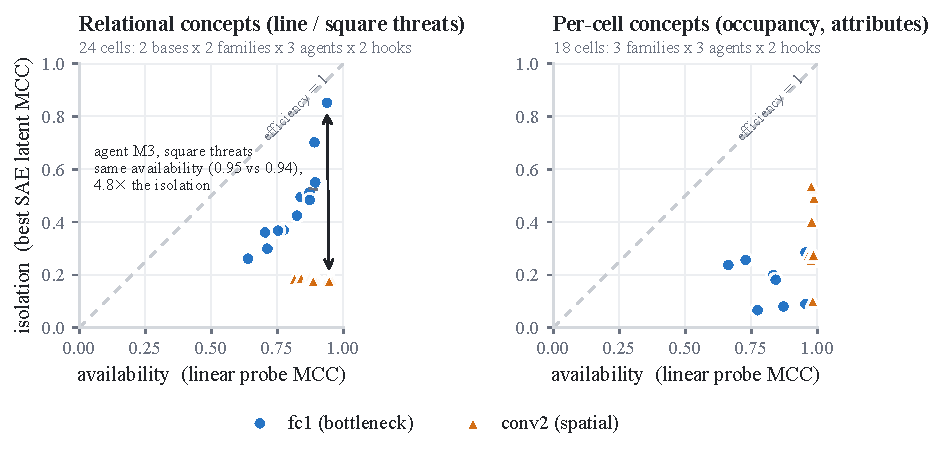
\includegraphics[width=0.9\linewidth]{fig_availability.pdf}
  \caption{Availability vs.\ isolation; the dashed diagonal is
    $\text{efficiency}=1$. \textbf{Left:} relational concepts. Both layers are
    far to the right---the information is there---but conv2 (triangles) is
    pinned near $I \approx 0.19$ regardless, while fc1 (circles) climbs toward
    the diagonal. \textbf{Right:} per-cell concepts, where the ordering
    reverses. The two lowest conv2 points are
    \texttt{offered\_piece\_attr}, whose base rate of $0.50$ makes it the
    trivial-baseline family.}
  \label{fig:avail}
\end{figure}

The natural reading of Table~\ref{tab:split} is that the bottleneck is where
threat information lives. The linear probe says otherwise
(Table~\ref{tab:avail}, Figure~\ref{fig:avail}). Over the state-threat cells,
\textbf{conv2 has the higher linear availability in 11 of 12}, while fc1 has the
higher efficiency in all 12. The extreme case is agent M3's square threats: the
two layers carry the concept \emph{equally well} ($A = 0.946$ at conv2 vs.\
$0.938$ at fc1, a difference of $0.008$) and their dictionaries differ by
\textbf{4.8$\times$} ($I = 0.178$ vs.\ $0.851$).

This is the paper's first observation. The information is not lost crossing the
bottleneck---a probe recovers it at $0.87$--$0.96$ on \emph{both} sides. What
changes is its \emph{form}: distributed across a spatial map at \texttt{conv2},
factored into individual directions at \texttt{fc1}. Note also how flat the
conv2 efficiency column is: $0.18$--$0.23$ across the twelve cells of
Table~\ref{tab:avail}, so whatever prevents atomisation there is insensitive
to how much of the concept is present. Along the competence axis
$\text{M1} \to \text{M2} \to \text{M3}$, by contrast, fc1 efficiency rises
$0.48 \to 0.59 \to 0.91$ on square threats and $0.41 \to 0.51 \to 0.62$ on line
threats, against conv2's flat $0.22 \to 0.18 \to 0.19$ and
$0.23 \to 0.19 \to 0.19$. Stronger agents do not merely encode threats
\emph{more}; they encode them in a form a flat dictionary can \emph{name}, and
only at the bottleneck.

\subsection{Retention: two failures that score the same}
\label{sec:retention}

Efficiency treats every low score alike. Retention does not. On the 114-cell
panel, pooled over three bases and all threat concepts:

\begin{center}
  \small
  \begin{tabular}{llrrrrr}
\toprule
agent & layer & $n$ & $R^2$ & $R^2_{\text{rand}}$ & retention & solo \\
\midrule
M1 & conv2 & 810 & 0.096 & 0.032 & 3.0$\times$ & 0.28 \\
M1 & fc1 & 810 & 0.163 & 0.031 & 5.3$\times$ & 0.43 \\
\addlinespace[2pt]
M2 & conv2 & 810 & 0.097 & 0.032 & 3.1$\times$ & 0.25 \\
M2 & fc1 & 810 & 0.260 & 0.028 & 9.2$\times$ & 0.58 \\
\addlinespace[2pt]
M3 & conv2 & 810 & 0.087 & 0.037 & 2.3$\times$ & 0.13 \\
\textbf{M3} & \textbf{fc1} & 810 & 0.565 & 0.037 & \textbf{15.2$\times$} & \textbf{0.92} \\
\bottomrule
\end{tabular}

\end{center}

At \texttt{conv2} the dictionary recovers $2.3$--$3.1\times$ the
untrained-network floor and concentrates $0.13$--$0.28$ of it, for \emph{every}
agent; at \texttt{fc1} both terms climb with competence, to $15.2\times$ and
$0.92$ on M3. Read against \S\ref{sec:availability}, where a probe reads state
threats off raw \texttt{conv2} activations at MCC $0.87$--$0.96$, this says
something sharper than ``conv2's dictionary is worse'': \textbf{the concept is
  in the layer and is not in the dictionary}, not even spread over 64 latents.
The convolutional failure is an encoding failure; only the bottleneck failure is
a factorisation failure in the sense \S\ref{sec:method} defines. Both score low
on isolation ($I = 0.18$ and $0.30$, far below what the probe predicts), so
isolation alone should not be used to choose a fix. A third case completes
the set and behaves exactly as the information account predicts: at
\texttt{conv2}, agent-relative concepts score low on \emph{availability} too
($0.338$, against $0.808$ at fc1 on M3's ``winnable square'' family). When a
layer genuinely lacks a
concept, availability drops as well; state threats do not behave that way, which
is the contrast \S\ref{sec:availability} rests on. Everything below
therefore concerns M3 / \texttt{fc1}, the one (agent, layer) where the
dictionary has resolved anything into atoms at all and so the only place where
``what does it do with the concepts it still misses'' is well posed.

\subsection{The residual wall is a disjunction wall}
\label{sec:disjunction}

\begin{table}[t]
  \centering
  \caption{Single-atom capture by concept shape, agent M3 / \texttt{fc1}, over
    all nine unsupervised dictionaries on that hook (3{,}209 concept verdicts).
    \emph{pinned} $=$ one location and one attribute pole. Within
    \textsc{count}, holding agent-relativity fixed, changing only the logical
    form takes capture from $81.2\%$ to $0.0\%$; holding form fixed and changing
    agent-relativity costs 2 points. solo $=$ concentration; $k_{90}$ and $R^2$
    are medians.}
  \label{tab:disj}
  \small
  \begin{tabular}{llcrrrrr}
\toprule
basis & concept shape & agent-rel. & $n$ & captured & solo & $k_{90}$ & $R^2$ \\
\midrule
state & pinned & no & 608 & 85.5\% & 0.974 & 1 & 0.763 \\
count & pinned & no & 532 & 81.2\% & 0.914 & 1 & 0.532 \\
count$^{-}$ & pinned & no & 532 & 62.2\% & 0.894 & 2 & 0.506 \\
count & pinned & yes & 532 & 79.0\% & 0.974 & 1 & 0.522 \\
count$^{-}$ & pinned & yes & 532 & 56.6\% & 0.862 & 2 & 0.419 \\
\midrule
\textbf{count} & \textbf{OR over 4 attributes} & no & 133 & \textbf{0.0\%} & 0.311 & 4 & 0.741 \\
\textbf{count$^{-}$} & \textbf{OR over 4 attributes} & no & 133 & \textbf{0.0\%} & 0.320 & 4 & 0.621 \\
\midrule
\textbf{agent-rel.} & \textbf{OR over 8 poles} & yes & 171 & \textbf{0.0\%} & 0.186 & 11 & 0.526 \\
\bottomrule
\end{tabular}

\end{table}

Our own earlier reading of these runs blamed \emph{agent-relativity}: the
concepts M3 / \texttt{fc1} still misses are the ones phrased from the mover's
point of view. That confounds three things, because a basis fixes logical form,
agent-relativity and prevalence at once. The comparison that separates them is
\emph{within} a single basis, and \textsc{count} supplies it---it contains both
logical shapes and both roles (Table~\ref{tab:disj}).

\textbf{Disjunction costs everything.} Within \textsc{count}, among the concepts
that are \emph{not} agent-relative, pinned ones are captured 81.2\% of the time
and disjunctive ones \textbf{0.0\%} (0 of 133);
\textsc{count}$^-$ repeats it independently on the opposite attribute poles,
$62.2\% \to 0.0\%$. Pooled over all four bases: 73.2\% (pinned, $n=2{,}736$)
against 0.0\% (disjunctive, $n=437$, zero exceptions).

\textbf{Agent-relativity costs almost nothing.} Within \textsc{count}, pinned
agent-relative concepts are captured 79.0\% against 81.2\% for pinned state
concepts---2 points, on 532 concepts each. Those agent-relative concepts read
the offered piece and have a median base rate of $0.0030$, and are still
captured four times in five. Pooled over bases the gap is 9 points. Whatever the
wall is, it is not agent-relativity.

\textbf{Nor is it prevalence.} A matched comparison settles it: restricting
both arms to a common base-rate window $[0.015, 0.050]$ leaves the effect
intact, 71.4\% captured for pinned ($n=868$) against \textbf{0.0\%} for
disjunctive ($n=437$). The direction runs the wrong way at the level of shape
too: the disjunctive concepts are the \emph{more common} (base rates
$0.0316$/$0.0226$) and the least captured, while the rarer pinned concepts
($0.0152$/$0.0029$) are captured 68--77\%. Critically, \textbf{the disjunctive
  concepts are not information-poor} (Figure~\ref{fig:disj}, left): they have the
\emph{highest} retention in the table---median $R^2 = 0.741$ for \textsc{count}'s
4-way disjunctions against $0.532$ for its pinned state concepts. The dictionary
knows the answer and has no atom for it.

\subsection{The mechanism, and what capacity does not fix}
\label{sec:mechanism}

\begin{figure}[t]
  \centering
  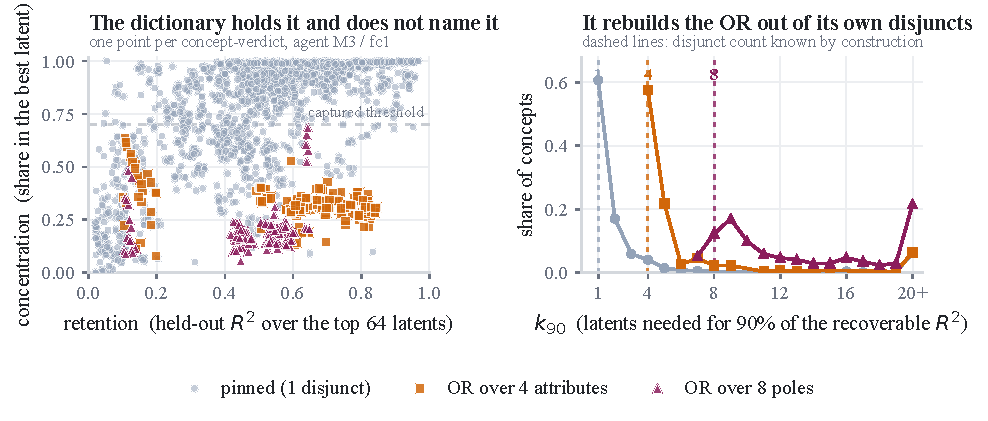
\includegraphics[width=0.9\linewidth]{fig_disjunction.pdf}
  \caption{Agent M3 / \texttt{fc1}, one point per concept verdict over nine
    unsupervised dictionaries. \textbf{Left:} the same geometry as
    Figure~\ref{fig:avail} one level down---the disjunctive concepts sit far to
    the right (the dictionary holds the signal) and low (no atom carries it),
    while the pinned cloud sits above the \texttt{captured} threshold.
    \textbf{Right:} $k_{90}$ against the disjunct count each concept has
    \emph{by construction} (dashed). The modal cost of a 4-way OR is exactly
    four latents and nothing is cheaper; the 8-way case peaks at 9 with a long
    tail (21.6\% at 20 or beyond, shown clipped).}
  \label{fig:disj}
\end{figure}

Because each ground-truth concept is a known Boolean function of the board, we
know how many disjuncts it has \emph{before looking at any dictionary}: one for
a pinned concept, four for an ``any threat here'' concept, eight for an
agent-relative ``winnable'' one. That makes $k_{90}$---normally too brittle to
read, because noise in the $R^2$ tail pushes the crossing right---usable as a
\emph{distribution} compared against a prediction it was not fitted to
(Figure~\ref{fig:disj}, right). The dictionary reconstructs a 4-way disjunction
from exactly four latents: over
its 266 such concepts the mode of $k_{90}$ is \textbf{4} (57.5\%) and
\textbf{not one is below 4}, against a mode of 1 (60.6\% of 2{,}736) for pinned
concepts. This is a direct observation of tiling rather than an inference from a
threshold---the prediction is fixed by the concept definitions, and the
measurement was free to land anywhere in $[1,64]$. The 8-way case is predicted
less sharply and behaves less sharply (mode 9, median 11, 5.3\% below
prediction, 21.6\% at 20 or beyond), the honest outcome for a concept that ORs
over a larger and rarer set.

The precondition bounds the claim: the signature appears \emph{only} on M3 /
\texttt{fc1}, the one cell where pinned concepts have modal $k_{90} = 1$.
Everywhere else pinned concepts already need 6--30 latents, so there are no
atoms for a disjunction to be tiled out of and $k_{90}$ is large and
unstructured. Tiling is conditional on atoms existing---and that precondition is
exactly what \texttt{conv2} and the two weaker agents lack
(\S\ref{sec:retention}).

\paragraph{Capacity does not fix it.} If the missing OR were a budget problem, a
larger dictionary would buy it. Holding recipe, seed, hook and agent fixed and
varying only $d_{\text{dict}}$ across $4{,}096 \to 16{,}384 \to 32{,}768$, the
share of agent-relative threat concepts coming out \emph{spread} is
$0.9565 \to 0.9565 \to 0.9565$---an 8$\times$ capacity increase moving the number
by $0.000$, with median concentration flat at $0.19$--$0.20$.

\subsection{Controls, robustness, and one cell we do not quote}
\label{sec:robustness}

\paragraph{The \texttt{captured} arm fires, and selection does not manufacture
  retention.} A three-way verdict is worthless if one arm never triggers. Across
the panel \texttt{captured} fires 2{,}265 times in 12{,}151 verdicts (18.6\%;
\texttt{spread} 74.6\%, \texttt{absent} 6.8\%), including the state basis's threat
categories at 85.5\% on M3 / \texttt{fc1}; the supervised positive control---slots
anchored to the agent-relative concepts by an auxiliary loss---comes out 16 of
23 \texttt{captured} at concentration $0.76$, against 0/23 for unsupervised
dictionaries on identical rows. All 114 cells carry 100\% random-control
coverage and none is provisional. Separately, ranking latents on rows that
overlap the rows $R^2$ is measured on is double-dipping that the permutation
null cannot see, since it shuffles labels \emph{after} selection; a
selection-aware null---permute first, then refit the whole pipeline---
returns $-0.0006$ to $-0.0013$ where the real values are $0.058$--$0.656$.
Selecting 64 of the 199--643 live latents buys no held-out $R^2$ from noise.

\paragraph{Repairing the weakest dictionary.} One panel member---M3's BatchTopK
dictionary at \texttt{conv2}---was degenerate (99.0\% dead latents, FVU $0.110$
against $0.043$/$0.051$ for the same recipe on the other agents), because the
dead-latent auxiliary loss of \citet{gao2024scaling} was applied to TopK but not
to BatchTopK in our code. A broken conv2 dictionary flatters our thesis, so we
retrained it (FVU $0.110 \to 0.0066$) and repeated the analysis. Of 15 families
\textbf{2 change sign, both per-cell, both toward the partition}; all twelve
relational families are unchanged, per-cell isolation recovers $\sim$5$\times$
($0.108 \to 0.527$), and square-threat isolation moves only $0.115 \to 0.178$
against fc1's $0.851$. Represented by its \emph{best} dictionary rather than its
worst, conv2 is demonstrably competent at per-cell concepts and still fails on
threats. All conv2 numbers above use the repaired dictionary except
Table~\ref{tab:split}, whose pre-repair split counts understate the partition.

\paragraph{Stability, and the one cell we do not quote.} Across a 4-condition
$\times$ 3-seed grid (1{,}764 concepts), 11.4\% of concept verdicts flip between
seeds, and 23 of 24 (agent, layer, basis) cells agree across three distinct
recipes. The exception is M3 / \texttt{conv2} / \textsc{agent-rel.}, where
retention sits at $1.6\times$ the untrained-network floor---close enough that
the \texttt{absent}/\texttt{spread} label is a coin flip
($0.39/0.65/0.39$ across seeds), so we quote no verdict for it. What all seven
of its runs do agree on is the measurement: $1.6\times$ the floor at
\texttt{conv2} with concentration $0.10$--$0.34$, against $14.6\times$ at
\texttt{fc1} on the same concepts and agent.

\section{Related work}
\label{sec:related}

Layer specialisation in game-playing networks is established.
\citet{lovering2022evaluation} find in AlphaZero-for-Hex that short-term
concepts probe best in final layers and long-term ones near mid-depth;
\citet{du2025gpt} report the SAE-based analogue in OthelloGPT, early layers
carrying static board attributes and deeper layers dynamic gameplay features.
Both compare \emph{probes} (or dictionaries) across layers. What we add is the
comparison of \emph{probe and dictionary on the same activations}, which
separates ``the layer knows it'' from ``the dictionary can name it.'' Under a
probe-only view \S\ref{sec:availability} is invisible: the probe alone says both
layers carry threats, the dictionary alone says only the bottleneck does.

Our disjunction result is, we think, feature absorption
\citep{chanin2024absorption} observed with exact ground truth. Absorption is
diagnosed in language models as a general feature (``starts with S'') failing to
fire because its children have taken the mass; here the general feature is a
disjunction we can write down, its children are the disjuncts we can also write
down, and we can count them---and its surviving an 8$\times$ capacity increase
reproduces their conclusion that size and sparsity are not the fix. The natural
response is a dictionary whose units may stand in a parent/child
relation---Matryoshka SAEs \citep{bussmann2025matryoshka}, hierarchical SAEs
\citep{muchane2025hierarchical}---and our measurement supplies an evaluation
those architectures currently lack: a concept set with a \emph{known} disjunct
count, where success means a parent atom firing on the union of children that
already exist and are already clean. This is a different brief from
multi-dimensional or manifold-aware dictionaries
\citep{engels2024notall,park2024geometry}, the right response to a concept
spread over an irreducible subspace---which also produces high availability with
low isolation, but not the tiled-by-disjunct signature of
\S\ref{sec:mechanism}. Finally, our per-family insistence echoes
\citet{karvonen2024measuring}: board-game ground truth is valuable precisely
because it is fine-grained, and averaging over the whole menu discards that.

\section{Discussion and limitations}
\label{sec:discussion}

A low SAE score is not self-interpreting. On these agents low isolation means
three different things, spanning a $3\times$ range ($I = 0.096$--$0.30$):
agent-relative concepts barely present in the convolutional layer, state
threats present in the layer but absent from its dictionary, and disjunctive
concepts present in the bottleneck's dictionary but split across their
disjuncts. Availability separates the first from the other two, retention the
second from the third, and only the third is a failure dictionary design can
address.
Reporting a probe baseline and a retention floor per concept family alongside
any SAE evaluation is cheap and changes which fix you reach for.

It also narrows the brief. The strongest agent's bottleneck already produces
clean single atoms for every pinned threat ($k_{90}=1$, median concentration
$0.93$); what is missing is not a better basis for those atoms but an
\emph{aggregating} unit above them. That points at the hierarchical arm of the
literature rather than the manifold arm, with a sharp, pre-registrable test: a
successful dictionary must move the 4-way disjunctions from $k_{90}=4$ to
$k_{90}=1$ without disturbing the pinned atoms they are built from.

\paragraph{Limitations.} \textbf{(i) Decodability, not causality}---every number
says a concept can be read out, not that the policy uses it; whether the clean
pinned atoms are the ones the policy consumes is untested. \textbf{(ii)
  Retention is measured over 64 of 4{,}096 latents}, so it lower-bounds what the
whole dictionary holds; a concept recoverable only from hundreds of latents
reads as low retention---the right reading for interpretability, not for
information content. \textbf{(iii) The tiling signature is conditional} on the
dictionary having resolved atoms at all, and holds on one (agent, layer) pair. \textbf{(iv) Linear
  availability only, and two layers rather than a depth sweep}. \textbf{(v) One game, one architecture
  family}; whether the partition and the disjunction wall transfer elsewhere is
untested, the strongest prior evidence being \citet{du2025gpt} and the
absorption literature's arrival at the same non-fix.

\bibliographystyle{plainnat}
\bibliography{refs}

\end{document}
